\chapter{Introduction}
\label{chp:introduction}

% printer: Tethered flight control of a small quadrotor robot for stippling \cite{galea_iros_2017}

%Example of energy harvesting: Prolonged energy harvesting for ingestible devices~\cite{plonski_tranro_2016}
%Drug delivery

% Estabish your territory

Miniature robots with limited capabilities in locomotion and sensing, can work together as a collective to achieve more than an individual could by itself.
The future potential of collectives of small robots, i.e. swarms, is widely recognized to have applications in surveillance, search and rescue operations, and exploration.
Swarms have also been proposed as a new form of user interface.
For instance, small robots can interact with users on tabletops~\cite{legoc_uist_2016}, unmodified clothing~\cite{dementyev_uist_2016} and can be an educational toy for kids~\cite{sony_toio_2017}, as seen in Figure \ref{fig:int_example_sui}.
%\hfill \break

% Establish nice
% Motivation for this work: Why do we want to remove the battery?

However, advanced swarms are still far from being applicable in real-world applications~\cite{barca_sekercioglu_2013}. 
One of the fundamental issues that needs to be addressed is related to the supply of energy.
Small lithium batteries are currently powering the robots and limit their operation time to only a few hours. 
To give a stark example, the energy density of batteries has improved less than one order of magnitude since 1945, while in comparison the energy efficiency of computing has improved 12 orders of magnitude~\cite{patel_pvc_2017}.
The last major advancement in battery technology is 25 years old and came with the introduction of Li-ion batteries.
Additionally, any new big improvements in energy density of batteries is not likely to happen anytime soon, as new battery technologies are often overhyped and slow to emerge~\cite{zachary_spec_2016}.
%	\hfill \break

%TODO introduce current research

% Propose a solution: Energy harvesting
% And discuss current solutions to autonomus operation / battery replenishment

Stable energy supplies are considered a requirement to allow long term persistent operation of robots.
%However, wireless sensor nodes that rely on energy harvesting have emerged.
%They are highly energy constrained, but fully eliminate the need for batteries~\cite{wisp5_wiki_2017}.
As of now, different replenishment methods for robot batteries are currently used, robots can be moved to a charging station, which leaves them non-operational.
At the same time, manual recharging or battery replacement results in a high strain on maintenance.
Therefore, relaxing the stable energy supply constraint by allowing a transient supply of harvested energy could be a potent area of research.

% 4 lines left!
\newpage

\begin{figure}
	\begin{subfigure}[b]{0.32\textwidth}
		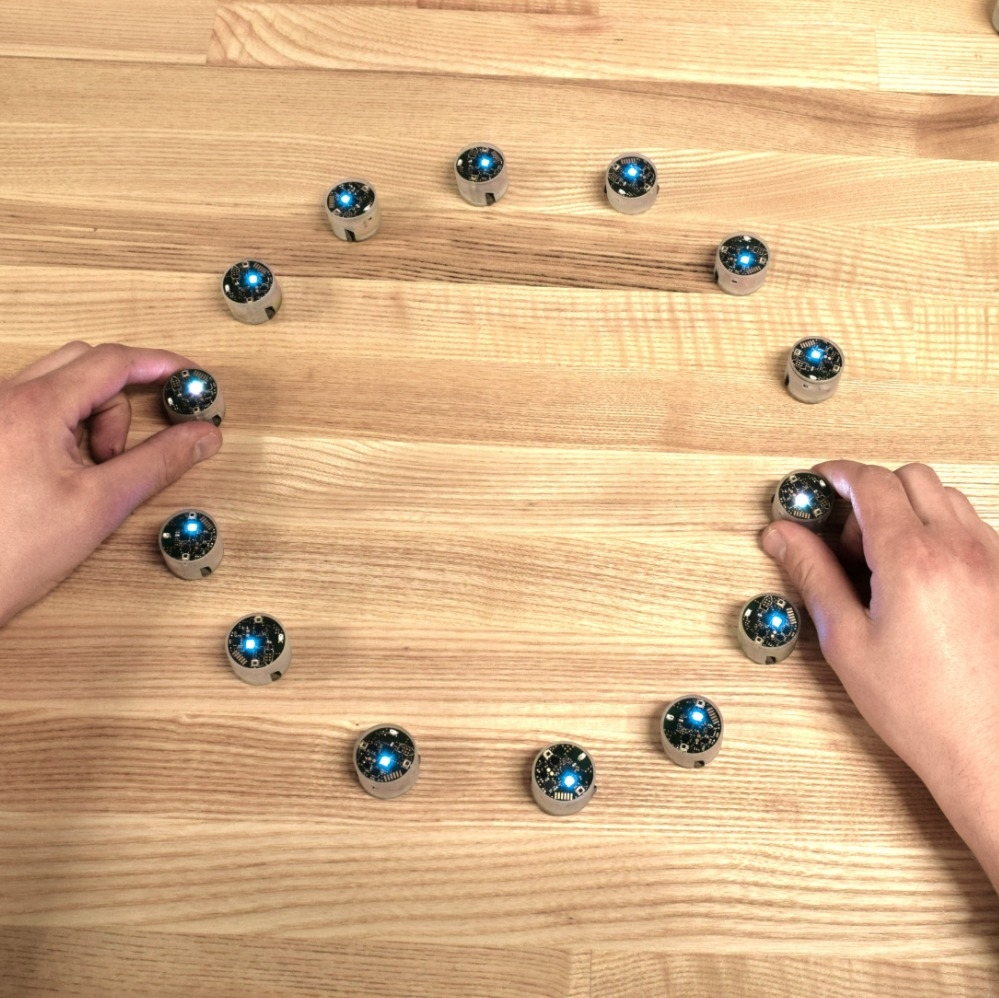
\includegraphics[width=\textwidth]{pics/zooids.jpg}
		\caption{Zooids~\cite{legoc_uist_2016}}
		\label{fig:int_zooids}
	\end{subfigure}
	\begin{subfigure}[b]{0.324\textwidth}
		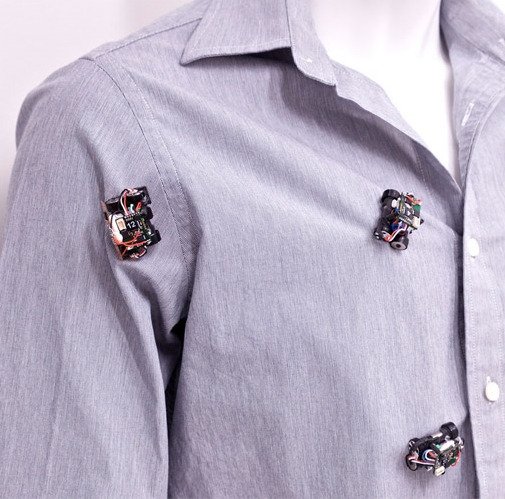
\includegraphics[width=\textwidth]{pics/rovables.jpg}
		\caption{Rovables~\cite{dementyev_uist_2016}}
		\label{fig:int_roverables}
	\end{subfigure}
	\begin{subfigure}[b]{0.323\textwidth}
		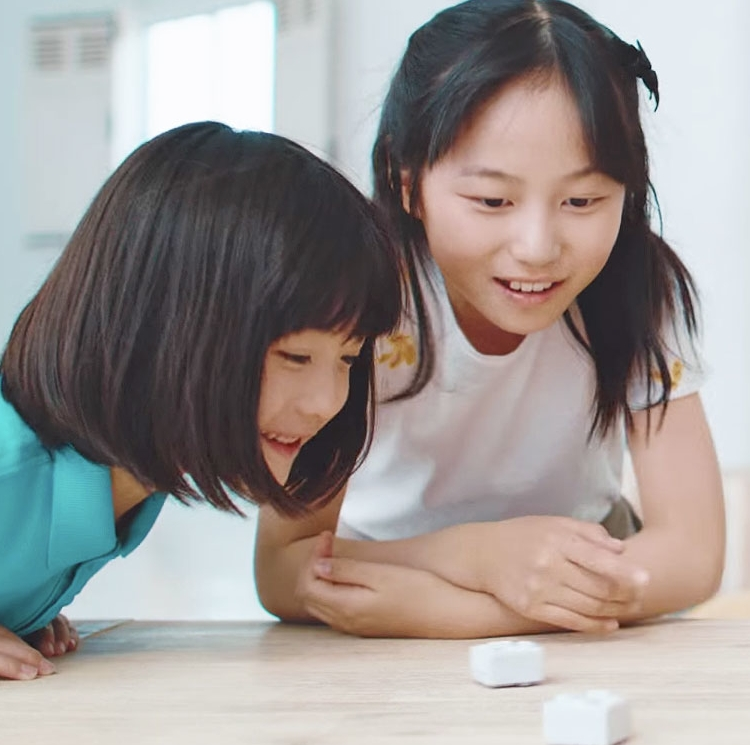
\includegraphics[width=\textwidth]{pics/toio.jpg}
		\caption{Sony Toio~\cite{sony_toio_2017}}
		\label{fig:int_toio}
	\end{subfigure}
	\caption{Current applications for small robotic platforms, ranging from swarm user interfaces and mobile wearables to educational toys for kids.}
	\label{fig:int_example_sui}
\end{figure}

\section{Problem statement}

% What why how

% Intermittently powered robots, that purely rely on harvested power are currently non existent.

% swarm robots ie kilobot operate form batteries -> need recharging -> move to tosti irond cannot be used while charging .

Replacing a battery with an energy harvesting system could make a robot self-sufficient and energy-autonomous. 
However, this introduces a new phenomenon that has to be taken into account: the \emph{intermittent availability} of energy produces frequent power interrupts.
The possibility of sudden power loss is currently not considered when developing control software for a robot, and for this reason can not be used without applying methods to preserve computation across power cycles.%adaption.
%\hfill \break

Furthermore, applicable sensors and/or sensing frequency may be constrained due to the limited energy budget.
The largest part of the energy budget is likely to be already consumed by the actuators that supply movement to the robot.
Not every actuator currently used for movement may be reliable and/or accurate under the frequent power interruption.
Therefore, the research question this work addresses is:

\begin{center}
	\textit{What is the effect of intermittency on the movement accuracy of a transiently-powered robot without external feedback?}
	%\textit{How to enable a transiently powered robot to operate autonomously?}
\end{center}

\section{Contributions}
The software controlling robots currently assumes that a task can only be completed if sufficient energy is left in the batteries, which inherently limits their operation time. 
This research explores the feasibility of a miniature battery-free robot, allowing persistent operation while being supplied by a small and intermittent source of energy.
%This is the first study of transiently powered robots, unaware of any platforms being implemented and are operating under the constant threat of power loss. 
The list of contributions is as follows:

\begin{enumerate}

%\item A simple model is developed showing the relation between the energy stored, weight of the robot, frequency of power cycles and distance covered with a single charge.

\item The design of a battery-free robot that purely operates from harvested energy, with basic capabilities allowing autonomous operation.

%TODO state results of implementation in contribution
\item The implementation of local movement feedback, that allows the robot to finish a movement across power cycles.

%\item Evaluation of the battery-free robot compared to a battery powered robot in terms of, weight, speed and accuracy of movement.

\end{enumerate}


\section{Thesis Outline}

The rest of the thesis is organized as follows: Chapter \ref{chp:related_work} provides background information and introduces the related work.
The preliminaries in design of the transiently-powered robot are presented in Chapter \ref{chp:preliminaries}.
In Chapter \ref{chp:design_and_implementation} the hardware design and software implementation are explained.
This is followed by a performance evaluation of the transiently-powered robot in Chapter \ref{chp:evaluation}.
Finally, Chapter \ref{chp:summary} concludes this thesis and proposes potential future work.



